\documentclass[12pt,a4paper]{article}
\usepackage{listings,chngcntr}
\usepackage{hyperref}% http://ctan.org/pkg/hyperref
\usepackage{paralist}
\usepackage{enumitem}% http://ctan.org/pkg/enumitem
\usepackage{amssymb}
\usepackage{amsmath,amsfonts,bm}
\usepackage{amsthm}
\newtheorem{theorem}{Theorem}[section]
\newtheorem{corollary}{Corollary}[theorem]
\newtheorem{lemma}[theorem]{Lemma}
\usepackage{url}
\usepackage{algorithm}
\usepackage[noend]{algpseudocode}
\usepackage{indentfirst}
\usepackage[percent]{overpic}
\makeatletter
\def\BState{\State\hskip-\ALG@thistlm}
\makeatother
\usepackage{mathtools}

\theoremstyle{definition}
\newtheorem{definition}{Definition}[section]
\usepackage{float}
\usepackage[utf8]{inputenc}
\usepackage{cleveref}
\crefname{section}{§}{§§}
\Crefname{section}{§}{§§}
\newcommand{\R}{\mathbb{R}}
 \usepackage{stmaryrd}
 \usepackage{graphicx}
 \usepackage{caption}
 \usepackage{subcaption}
 \usepackage[english]{babel}

\usepackage{listings}
\usepackage{color}
\usepackage{graphicx, epstopdf}
\usepackage{listings}
\lstset{language=Python}
\renewcommand{\sectionautorefname}{\S}
\setlength{\topmargin}{0.0in}
\setlength{\oddsidemargin}{0.33in}
\setlength{\textheight}{9.0in}
\setlength{\textwidth}{6.0in}
\renewcommand{\baselinestretch}{1.25}
\setlist[itemize]{noitemsep, topsep=0pt}
\definecolor{codegreen}{rgb}{0,0.6,0}
\definecolor{codegray}{rgb}{0.5,0.5,0.5}
\lstset{
	frame=single,
	numbers = left,
	basicstyle=\fontsize{9}{11}\ttfamily\linespread{0.85}\ttfamily,
    breaklines=true
}
\title{Hierarchical Model Adaptivity}
\author{Author: Georgios Sialounas}

\begin{document}
\counterwithin{lstlisting}{section}
\maketitle
\thispagestyle{empty}
\newpage
\tableofcontents
\thispagestyle{empty}
\newpage
\setcounter{page}{1}


\section{Introduction and Motivation}

It is often the case when modelling physical phenomena that we need to solve a complicated Partial Differential Equation (PDE).  Such models may result in systems of equations which are computationally expensive to solve.  One way to overcome this difficulty is to use some physical reasoning to simplify the model of equations into a simpler model.  The justification is that the simpler model describes the physical system adequately even with the loss of information incurred through the simplification.  

Situations calling for such simplifications abound.  As an example consider oceanic flow: very close to bottom of the ocean, which we suppose is a fixed boundary, one will need to make use of the Navier-Stokes equations in order to accurately flow characteristics in the boundary layer.  Far-afield however, where viscocity is not important, one can accurately describe the flow with the Euler equations.  

The natural problem with this approach are cases in which we actually do need to make use of the complex model in a small part of the domain in order to produce reliable, accurate results.   The mathematical challenge that arises is in the coupling of the simple and complex models so that we retain the savings from using the former in the majority of the domain and the accuracy from using the latter in specific parts of the domain as necessary.

This model refinement can be based on knowledge available $\textit{a priori}$, which informs the decomposition of the domain or on results made available $\textit{a posteriori}$, i.e. during the computation.

The aim of this project will be to develop a strategy to adaptively choose an appropriate model to approximate over specific parts of the domain in real time.  The specific example we will considered is flow governed by Stokes's equations, to be reduced to the vectorial Laplacian in parts of the domain where pressure is constant.  The reduction will be based on localised error estimates.  We will examine the errors due to numerical approximation and also due to the model reduction itself.

The rest of the project is structured as follows.  In \S \ref{sec_back} we present work that has been previously done in the area.  In \S \ref{sec_mathform} we describe Stokes's equations, introduce their weak form and show that the resulting problem is well-posed.  In \S \ref{sec_adaptivity} we  describe adaptivity and how it will be implemented in this project in greater depth.  In \S \ref{sec_numerics} we present some preliminary results that are produced with the Deal II software (see \cite{BangerthHartmannKanschat2007}), which  will be used for the numerical implementation component of the project.  We conclude the report in \S \ref{sec_conclusion}, where we also discuss the next steps.

\section{Background}\label{sec_back}
In this section I will present some of the work that has already been done on adaptivity.

\section{Mathematical Formulation}\label{sec_mathform}
In this section we present Stokes's equations and their weak form.   These are used to describe very slow flows (in the limit as the Reynold's number tends to zero).  Such flows might include the motion of the fluid very close to a solid boundary or the flow of magma in the Earth's mantle.  
\subsection{Stoke's Problem}
Stoke's problem in a domain $\Omega = \left[0,1\right]^2 \subset \mathbb{R}^2$ involves finding $\left(\textbf{u},p\right)$ such that:
\begin{equation}\label{stokes_eq}
\begin{aligned}
	-\Delta\textbf{u} + \nabla p &= \textbf{f} \\ 
	\nabla\cdot \textbf{u}&= 0\\ 
\textbf{u}|_{\partial\Omega}&=0 
\end{aligned}
\end{equation}
where boldface indicates vectors.  In (\ref{stokes_eq}), $\textbf{u},\, \textbf{f}$ and $p$ represent the velocity, the forcing and the pressure respectively.  In this case we have used zero (Dirichlet) boundary conditions. 
\subsection{Weak Formulation}\label{weak-form-stokes}
We obtain the weak form of (\ref{stokes_eq}) by multiplying the equations with test functions $\textbf{v}$ and $q$ and integrating by parts.  This gives us:
\begin{eqnarray}\label{form-a}
	a\left(\textbf{u},\textbf{v}\right) + b\left(\textbf{v},p\right) &=& F\left(\textbf{v}\right)\quad \forall 
\textbf{v} \in \mathbb{V} \text{ and} \\\label{form-b}
	b\left(\textbf{u},q\right)&=&0 \quad \quad\quad\forall q \in \mathbb{P},
\end{eqnarray}
where 
\begin{eqnarray}\label{weak-a}
	a\left(\textbf{u},\textbf{v}\right)&=&\int_{\Omega}\nabla \textbf{u} : \nabla \textbf{v}, \\\label{weak-b}
	b\left(\textbf{v},q\right) &=& \int_{\Omega}-q\left(\nabla \cdot \textbf{v}\right) \text{ and}\\\label{weak-F}
    F\left(\textbf{v}\right) &=& \int_{\Omega}\textbf{f}\cdot \textbf{v} ,
\end{eqnarray}
The function spaces $\mathbb{V}$ and $\mathbb{P}$ are defined as follows:
\begin{eqnarray}\label{fspace_V}
\mathbb{V}&=&\textbf{H}^1_0\left(\Omega\right)^2\text{, with norm: } \left|\textbf{v}\right|_{1}=\left|\left|\nabla\textbf{v}\right|\right|_{L^2\left(\Omega\right)}, \\\label{fspace P}
\mathbb{P}&=&L^2_0\left(\Omega\right)=\left\lbrace q\in L^2\left(\Omega\right): \int_\Omega q=0\right\rbrace\text{, with norm: } \left|\left|q\right|\right|_{L^2\left(\Omega\right)}
\end{eqnarray}
Note that by the $(\cdot)^2$ in $\textbf{H}^{1}_{0}\left(\Omega\right)^2$ we indicate that we are dealing with vectorial functions with two components. Henceforth, we will adopt the notation $\left|\textbf{u}\right|_1$ and $\left|\left|q\right|\right|_{L^2}$ for the norms pertaining to the function spaces specified in (\ref{fspace_V}) and (\ref{fspace P}).  The reader should take it for granted that the quantity is taken over the domain $\Omega$ rather than just, say, the boundary $\partial \Omega$, unless the context explicitly specifies otherwise.
\subsection{Well Posedness}\label{sec_wellposed}
We will introduce some notation that will be used for the analysis in this section.  We will adopt the same notation as \cite{Chen2016} for ease of cross-checking, as the analysis in this section relies heavily on results presented therein. 
We will also be frequently making use of the symbol
\begin{equation}
	\lesssim \nonumber,
\end{equation}
which we we will define as follows: if $a\lesssim b$ this means $a\leq C\cdot b$, with $C>0$.  We will also define two important concepts in terms of proving well-posedness: coercivity and boundedness.
\theoremstyle{definition}
\begin{definition}{Coercivity and boundedness} (see \cite{brenner2007mathematical}: Definition 2.5.2)
	An (abstract) bilinear form $a\left(\cdot,\cdot\right)$ on a normed linear space $H$ is said  to be bounded (or continuous) if $\exists C > 0$ such that
	\begin{equation}
		\left|a\left(u,v\right)\right|\leq C \left|\left|u\right|\right|_H\left|\left|v\right|\right|_H \quad \forall u,v \in H\nonumber
	\end{equation}
	and coercive on $V\subset H$ if $\exists$ $\alpha > 0$ such that
	\begin{equation}
	a\left(v,v\right)\geq \alpha \left|\left|v\right|\right|_H^2\quad \forall v \in V\nonumber.
	\end{equation}
\end{definition}
\subsubsection{PDE}\label{PDE_cont}
There are four components to proving the well-posedness of (\ref{stokes_eq}):
	 \begin{eqnarray}\label{coerc_a}
	\inf_{\textbf{u}\in \mathbb{V}}\sup_{\textbf{v}\in \mathbb{V}}\frac{a\left(\textbf{u},\textbf{v}\right)}{\left|\textbf{u}\right|_1 \left|\textbf{v}\right|_1}&=&\alpha>0,\\\label{coerc_b}
			\inf_{q\in \mathbb{P}}\sup_{\textbf{u}\in \mathbb{V}}\frac{b\left(\textbf{u},q\right)}{\left|\textbf{u}\right|_1 \left|\left|q\right|\right|_{L^2}}&=&\beta>0,\\\label{cont_a}
		a\left(\textbf{u},\textbf{v}\right)&\leq& C_a\left|\textbf{u}\right|_1\left|\textbf{v}\right|_1,\, \forall \textbf{u},\textbf{v} \in \mathbb{V}\text{ and}\\\label{cont_b}
		b\left(\textbf{u},q\right)&\leq& C_b\left|\textbf{u}\right|_1\left|\left|q\right|\right|_{L^2},\,\forall \textbf{u} \in \mathbb{V},\, q \in \mathbb{P}.
	\end{eqnarray}
Briefly, (\ref{coerc_a}) and (\ref{coerc_b}) correspond to the stability of the bi-linear forms specified in (\ref{weak-a}) and (\ref{weak-b}) respectively, while (\ref{cont_a}) and (\ref{cont_b}) correspond to their boundedness, in the same order. It is worth noting that (\ref{weak-b}) is perhaps more widely known as the $\textit{inf-sup}$ condition (see \cite{brenner2007mathematical}: \S 12). It is relatively easier to show that conditions (\ref{weak-a}), (\ref{cont_a}) and (\ref{cont_b}) hold than to show (\ref{weak-b}) holds, so we will start with the latter.  However, firstly we will introduce a result that implies (\ref{weak-b}) holds.  The result can be found in \cite{Chen2016} as Lemma 1.4.
\begin{lemma}\label{Lemma_equiv}
	For any $q\in L^2_0\left(\Omega\right), \exists \textbf{v}\in \textbf{H}^1_0\left(\Omega\right)$ such that
	\begin{equation}
		\nabla \cdot \left(\textbf{v}\right) = q \text{ and } \left|\textbf{v}\right|_1 \lesssim \left|\left|q\right|\right|_{L^2}\nonumber.
	\end{equation}
	Consequently, the inf-sup condition, (\ref{coerc_b}), holds.
\end{lemma}
\begin{proof}
	See \cite{Chen2016}: Lemma 1.4
\end{proof}
We will use the statement of Lemma \ref{Lemma_equiv} to show it implies (\ref{coerc_b}).  Consider (\ref{weak-b}).  We choose $\textbf{v}$ so that the result in Lemma (\ref{Lemma_equiv}) holds. We will label this $\textbf{v}$ as $\textbf{v}_q$ to remember the dependence on $q$.   Hence
\begin{eqnarray}
b\left(\textbf{v}_q,q\right) &=& \left|\left|q\right|\right|_{L^2}^2 \quad\text{by Lemma \ref{Lemma_equiv}  and defn of } \nonumber \left|\left|\cdot\right|\right|_{L^2},\\
&\gtrsim& \left|\left|q\right|\right|_{L^2} \left|\textbf{v}_q\right|_1\quad \text{by Lemma \ref{Lemma_equiv}}.\nonumber
\end{eqnarray}
Now, assuming that $\left|\textbf{v}_q\right|_1$, which we assume not to be zero and take the supremum over $\textbf{v}\in \mathbb{V}$ to get:
\begin{equation}
\sup_{\textbf{0}\neq\textbf{v}\in \mathbb{V}}\frac{b\left(\textbf{v},q\right)}{\left|\textbf{v}\right|_1} \gtrsim \left|\left|q\right|\right|_{L^2}.\nonumber
\end{equation}
Now we divide throughout by $\left|\left|q\right|\right|$, which we also assume not to be equal to zero, and take the $\inf$ of that, which we can do since the inequality is required to hold for all $q\in \mathbb{P}$:
\begin{equation}
\inf_{q\in \mathbb{P}}\frac{1}{\left|\left|q\right|\right|_{L^2}}\sup_{\textbf{v}\in \mathbb{V}}\frac{b\left(\textbf{v},q\right)}{\left|\textbf{v}\right|_1} \gtrsim 1 \nonumber.
\end{equation}
Lastly, since $q$ does not depend on the choice of $\textbf{v}$, we can move it inside the supremum to obtain the required result, i.e. (\ref{coerc_b}) $\qedsymbol$ .  

Next, we show that (\ref{coerc_a}) holds.  This is implied by the fact that (\ref{weak-a}) is coercive:
\begin{eqnarray}
		a\left(\textbf{u},\textbf{u}\right)&=&\int_{\Omega}\nabla \textbf{u} : \nabla \textbf{v}\;\mathrm{d}x,\nonumber\\
		&=&\int_{\Omega}\sum_{i}\nabla u_i \cdot \nabla u_i\;\mathrm{d}x\text{ and}\nonumber\\
		&=&\left|\textbf{u}\right|_1^2,\nonumber
\end{eqnarray}
which is the coercivity condition with equality and $\alpha = 1$.  Now we show that  the coercivity of $a\left(\cdot,\cdot\right)$ implies (\ref{coerc_a}.  Since $a\left(\cdot,\cdot\right)$ is coercive, we have that
\begin{equation}
a\left(\textbf{u},\textbf{u}\right)\geq \alpha  \left|\textbf{u}\right|_1^2 \nonumber.
\end{equation}
We divide throughout by $\left|\textbf{u}\right|_1$, which we assume not to be zero. 
\begin{equation}
\frac{a\left(\textbf{u},\textbf{u}\right)}{\left|\textbf{u}\right|_1}\geq \alpha \left|\textbf{u}\right|_1 \nonumber
\end{equation}
 Then we take the supremum on the left-hand side over all $\textbf{v}\in\mathbb{V}$:
 \begin{equation}
 \sup_{\textbf{v}\in \mathbb{V}}\frac{a\left(\textbf{u},\textbf{v}\right)}{\left|\textbf{v}\right|_1}\geq \alpha \left|\textbf{u}\right|_1\nonumber
 \end{equation}
 Since this result hold for any $\textbf{u}\in \mathbb{V}$ then it also holds for the infimum over $\textbf{u}$:
\begin{equation}
\inf_{\textbf{u}\in \mathbb{V}}\sup_{\textbf{v}\in \mathbb{V}}\frac{a\left(\textbf{u},\textbf{v}\right)}{\left|\textbf{v}\right|_1\left|\textbf{u}\right|_1} \geq \alpha>0\nonumber.
\end{equation}
Lastly, (\ref{cont_a}) and (\ref{cont_b}) follow from an application of the Cauchy-Schwarz inequality on the corresponding bilinear forms.
\subsubsection{Discrete form of the $\textit{inf-sup}$ condition}\label{PDE_disc}
In \S \ref{PDE_cont} we consider (\ref{weak-a}) and \ref{weak-b} in the setting of infinite-dimensional function spaces.  In practice we will be dealing with a finite-dimensional version of these.  Hence, we need to show that the discrete, finite-dimensional problem is also well-posed:
\begin{eqnarray}
		a\left(\textbf{u}_h,\textbf{v}\right) + b\left(\textbf{v},p_h\right) &=& F\left(\textbf{v}\right)\quad \forall 
	\textbf{v} \in \mathbb{V}_h \text{ and} \\
	b\left(\textbf{u}_h,q\right)&=&0 \quad \quad\quad\forall q \in\mathbb{P}_h,
\end{eqnarray}
where $\mathbb{V}_h\subset\mathbb{V}$ and $\mathbb{P}_h\subset\mathbb{P}$.  In this case, the discrete version of the $\textit{inf-sup}$ condition, (\ref{coerc_b}), is given by
\begin{equation}\label{coerc_b_disc}
	\inf_{q\in \mathbb{P}_h}\sup_{\textbf{u}\in \mathbb{V}_h}\frac{b\left(\textbf{u},q\right)}{\left|\textbf{u}\right|_1 \left|\left|q\right|\right|_{L^2}}=\beta>0.
\end{equation}
In order to show that (\ref{coerc_b_disc}) holds we will first introduce some results and definitions. Firstly, we define the Fortin operator:
\theoremstyle{definition}
\begin{definition}{Fortin Operator} (\cite{Chen2016}: Definition 2.1)\label{Fortin_defn}
	A linear operator $\Pi_h: \mathbb{V} \rightarrow \mathbb{V}_h$ is called a Fortin Operator if:
	\begin{enumerate}
	\item$b\left(\Pi_h v, q_h\right)=b\left(v, q_h\right)\quad \forall q_h \in \mathbb{P}_h,$
	\item $\left|\left|\Pi_h v\right|\right|_{\mathbb{V}}\leq C\left|\left|v\right|\right|_\mathbb{V}.$
	\end{enumerate}
\end{definition}
\begin{theorem}\label{theorem_inf_sup_disc}
	Assume the continuous inf-sup condition, (\ref{coerc_b}) holds and there exists a Fortin Operator $\Pi_h$, then the discrete inf-sup condition (\ref{coerc_b_disc}) holds.
\end{theorem}
\begin{proof}
	Since the continuous $\textit{inf-sup}$ condition (\ref{coerc_b}) holds then we know from Lemma \ref{Lemma_equiv} that for any $q\in \mathbb{P}_h \subset \mathbb{P}$ $\exists \textbf{v}\in \mathbb{V}$ such that
	\begin{equation}
		b\left(\textbf{v}, q_h\right)\geq \beta \left|\textbf{v}\right|_1\left|\left|q_h\right|\right|_{L^2} \text{ and } \left|\textbf{v}\right|_1 \lesssim \left|\left|q_h\right|\right|_{L^2}. \nonumber
	\end{equation} 
We have assumed that $\exists$ $\Pi_h$ and from item 1 of this definition we can choose $\textbf{v}=\Pi_h \textbf{v}\in \mathbb{V}_h$ such that
\begin{equation}
	b\left(\Pi_h\textbf{v},q_h\right) =b \left(\textbf{v},q_h\right). \nonumber
\end{equation}
Since (\ref{coerc_b}) holds, we have that
\begin{eqnarray}
b \left(\textbf{v},q_h\right)&\geq& \beta \left|\textbf{v}\right|_1\left|\left|q_h\right|\right|_{L^2} \nonumber \\
&\geq& \frac{\beta}{C} \left|\Pi_h\textbf{v}\right|_1\left|\left|q_h\right|\right|_{L^2}\quad \text{from item 2 of Definition \ref{Fortin_defn}}. \nonumber
\end{eqnarray}
Hence, the discrete $\textit{inf-sup}$ condition holds.
\end{proof}
\subsubsection{Stability bounds}
In the case of the continuous problem, we use (\ref{coerc_a})-(\ref{cont_b}) to show that a solution to (\ref{stokes_eq}) is stable. Firstly, we let 
\begin{equation}
	\textbf{v}=\textbf{u},\, q =p
\end{equation}
so that (\ref{form-a}) and (\ref{form-b}) respectively become
\begin{eqnarray}\label{nform-a}
\int_{\Omega}\nabla \textbf{u} : \nabla \textbf{u}+\left(\nabla \cdot \textbf{u}\right)p\;\mathrm{d}x  &=&\int_{\Omega}\textbf{f}\cdot \textbf{u} \;\mathrm{d}x
 \text{ and} \\\label{nform-b}
\int_{\Omega}\left(\nabla \cdot \textbf{u}\right)p\;\mathrm{d}x&=& 0.
\end{eqnarray}
We now substitute (\ref{nform-b}) in (\ref{nform-a}) to obtain
\begin{equation}
\int_{\Omega}\nabla \textbf{u} : \nabla \textbf{u}\;\mathrm{d}x  =\int_{\Omega}\textbf{f}\cdot \textbf{u} \;\mathrm{d}x.
\end{equation}
Notice that the left-hand side is equal to $\left|\textbf{u}\right|_1^2$.  We apply the Cauchy-Schwarz inequality to get
\begin{equation}\label{cauchy-a}
\left|\textbf{u}\right|_1^2\leq\left|\left|\textbf{f}\right|\right|_{L^2}\left|\left|\textbf{u}\right|\right|_{L^2}.
\end{equation}
We would now like to bound the right-hand side such that we obtain a bound based on problem data.  We can do this by using Poincar\'e's inequality:
\begin{equation} 
\left|\left|\textbf{u}\right|\right|_{L^2}\leq C_p\left|\textbf{u}\right|_1\text{, } C_p>0
\end{equation}
Interested readers can find further details on this inequality and its applicability  in (e.g.) \cite{brenner2007mathematical}: \S 5.3.  We use this in (\ref{cauchy-a}) to get
\begin{equation}\label{cauchy-b}
\left|\textbf{u}\right|_1^2\leq C_p\left|\left|\textbf{f}\right|\right|_{L^2} \left|\textbf{u}\right|_1.
\end{equation}
Hence we obtain a bound on $\left|\textbf{u}\right|_1$, 
\begin{equation}\label{bound-u-cont}
\left|\textbf{u}\right|_1\leq C_p\left|\left|\textbf{f}\right|\right|_{L^2}.
\end{equation}
We now try to obtain a bound for $\left|\left|p\right|\right|_{L^2}$ in terms of the problem data, $\textbf{f}$.  The $inf-sup$ condition, (\ref{coerc_b}), implies that
\begin{equation}\nonumber
\beta \left|\left|q\right|\right|_{L^2}\leq \sup_{\textbf{v}\in \mathbb{V}, \,\left|\textbf{v}\right|_{L^2}\leq1}  b\left(\textbf{v},q\right)\quad  \forall q \in L^2
\end{equation}
We now choose $q=p$, which gives 
\begin{eqnarray}\nonumber
\beta \left|\left|p\right|\right|_{L^2} &\leq& \sup_{\textbf{v}\in \mathbb{V}, \,\left|\textbf{v}\right|_1\leq1}  b\left(\textbf{v},p\right)\\\nonumber
&=& \sup \left(\int_{\Omega}\textbf{f}\cdot\textbf{v} -\nabla\textbf{u}:\nabla\textbf{v}\right)\\\nonumber
\text{Cauchy-Schwarz: }&\leq& \sup \left(\left|\left|\textbf{f}\right| \right|_{L^2} \left|\left|\textbf{v}\right|\right|_{L^2}+\left|\textbf{u}\right|_1 \left|\textbf{v}\right|_1\right)\\\nonumber
\text{Poincar\'e's: }&=&\sup \left[\left(C_p\left|\left|\textbf{f}\right| \right|_{L^2}+ \left|\textbf{u}\right|_1\right) \left|\textbf{v}\right|_1\right] \\\nonumber
\left|\textbf{v}\right|_1\leq 1\text{:} &\leq&C_p\left|\left|\textbf{f}\right| \right|_{L^2}+ \left|\textbf{u}\right|_1\\\nonumber
\text{Using }\left(\ref{bound-u-cont}\right):&\leq&2C_p\left|\left|\textbf{f}\right| \right|_{L^2}
\end{eqnarray}
Hence, we have also obtained a stability bound on $\left|\left|p\right|\right|_{L^2}$ :
\begin{equation}\label{bound-p-cont}
\left|\left|p\right|\right|_{L^2} \leq \frac{2C_p}{\beta}\left|\left|\textbf{f}\right|\right|_{L^2}.
\end{equation}
Bounds (\ref{bound-u-cont}) and (\ref{bound-p-cont}) show that the solution to (\ref{stokes_eq}) is stable:
\begin{equation}
\left|\textbf{u}\right|_1+\left|\left|p\right|\right|_{L^2} \leq\left( C_p+\frac{2C_p}{\beta}\right)\left|\left|\textbf{f}\right|\right|_{L^2}.
\end{equation}
In conclusion, in this section we have shown that our problem has a unique, stable solution.
\subsubsection{Linear System}
In here I will present the linear system arising from the PDE and explain what we will need for it to have a unique solution (I will also show that analysis with the Shur complement etc.)
\section{Adaptivity}\label{sec_adaptivity}
The main objective in this project is to develop a strategy for switching between Stokes equation and Poisson equation in different parts of our domain.  In this section we will consider a domain which is divided into sub-domains based on the equations governing the flow in each subdomain.  Specifically, we want to find $\left(\textbf{u},p\right)$ that satisfies:
\begin{equation}
	\begin{aligned}\label{stokes_eq_adapt}
\text{In $\Omega_{1}$: }  -\Delta\textbf{u} + \nabla p &= \textbf{f} \\ 
	\nabla\cdot \textbf{u}&= 0
	\end{aligned}
\end{equation}
\begin{equation}\label{poisson_eq_adapt}
\text{In $\Omega_{2}$: }-\Delta\textbf{u}= \textbf{f}
\end{equation}
with boundary conditions given by
\begin{equation}\label{bc_adapt}
	\textbf{u}= 0 \text{\quad on $\partial \Omega$}.
\end{equation}
The domain is shown in Figure \ref{fig_domain}.  Naturally, we would like to know whether the problem given by (\ref{stokes_eq_adapt})-(\ref{bc_adapt}) has a unique, stable solution.  In order to do this we will first derive the variational form for (\ref{stokes_eq_adapt})-(\ref{bc_adapt}) and then we will repeat some of the procedures from \S \ref{sec_wellposed} to show that our problem is well-posed.
\begin{figure}[H]
	\centering
	\begin{overpic}[width=0.6\textwidth]{domain}
		\centering
		\put (20,30) {\huge$\displaystyle\Omega_{1}$}
		\put (70,30) {\huge$\displaystyle\Omega_{2}$}
		\put (50,30) {\huge$\displaystyle\mathcal{I}$}
		\put (87,52) {\huge$\displaystyle\partial \Omega$}
		\put (54,11) {\huge$\displaystyle \textbf{n}_1$}
		\linethickness{1pt}
		\put(47,10){\color{red}\vector(1,0){10}}
		\put (54,11) {\huge$\displaystyle \textbf{n}_1$}
		\linethickness{1pt}
		\put(99,30){\color{red}\vector(1,0){10}}
		\put (106,31) {\huge$\displaystyle \textbf{n}_2$}
	\end{overpic}
	\caption{Domain for the adaptive problem, with subdomains $\Omega_{1}$ (Stokes equations), $\Omega_{2}$ (Poisson equation)and boundary $\partial \Omega$ with homogeneous Dirichlet boundary conditions. The interface $\mathcal{I}$ separates the part of the domain where we solve each of the two problems.  The unit vectors $\textbf{n}_1$ and $\textbf{n}_2$ are the outward normals to $\Omega_{1}$ and $\Omega_{2}$ respectively.}
	\label{fig_domain}
\end{figure} 
\subsection{Variational Form}
In this section we derive a variational form for (\ref{stokes_eq_adapt})-(\ref{poisson_eq_adapt}).  We begin by testing the first and second equations in  (\ref{stokes_eq_adapt}) with test functions $\textbf{v}\in \mathbb{V}$ and $q\in \mathbb{P}$, where  $\mathbb{V}$ and $\mathbb{P}$ have been defined in (\ref{fspace_V}) and (\ref{fspace P}) respectively. We integrate the resulting equations by parts to obtain:
\begin{equation}\label{weak_stokes_1}
\begin{aligned}
\int_{\Omega_1}\nabla \textbf{u}^{\left(1\right)} : \nabla \textbf{v}+p\left(\nabla \cdot \textbf{v}\right) +\int_{\mathcal{I}} p\textbf{v}\cdot \textbf{n}_1-\textbf{v}\cdot\left(\textbf{n}_1\cdot\nabla\textbf{u}^{\left(1\right)}\right) &=\int_{\Omega_1}\textbf{f}\cdot \textbf{v}  \quad \forall  \textbf{v}\in \mathbb{V}\\
\int_{\Omega_1}q\left(\nabla \cdot \textbf{u}^{\left(1\right)}\right) &= 0\quad \forall q\in \mathbb{P},
\end{aligned}
\end{equation}
for subdomain $\Omega_1$ and
\begin{equation}\label{weak_poisson}
\int_{\Omega_2}\nabla \textbf{u}^{\left(2\right)} : \nabla \textbf{v} - \int_{\mathcal{I}} \textbf{v}\cdot\left(\textbf{n}_2\cdot\nabla\textbf{u}^{\left(2\right)}\right)= \int_{\Omega_2}\textbf{f}\cdot \textbf{v}  \quad \forall  \textbf{v}\in \mathbb{V}
\end{equation}
for $\Omega_2$, where the unit vectors $\textbf{n}_1$ and $\textbf{n}_2$ are the outward normals to $\Omega_{1}$ and $\Omega_{2}$ respectively and $\nabla \textbf{u}^1$ and $\nabla \textbf{u}^2$ are the flux gradients in the two subdomains. Notice that the boundary integrals are taken over $\mathcal{I}$ rather than over $\partial \Omega_{1}$ and $\partial \Omega_{2}$ because $\textbf{v}=\textbf{0}$ on $ \partial \Omega = \partial \Omega_1\cup \Omega_{2}\setminus \mathcal{I}$.   

Before we proceed, we introduce a jump operator, which is simply a notational convenience for expressing the jump of a quantity across an discontinuity.  Consider a (vector) quantity, $\textbf{b}$, whose values at either side of a curve $e$ in $\Omega$ are $\textbf{b}^{\left(1\right)}$ and $\textbf{b}^{\left(2\right)}$.  In this case, $e = \mathcal{I}$, the interface between the two subdomains.  Then, the jump accross $\mathcal{I}$ is given by:
\begin{equation}
\llbracket \textbf{u} \rrbracket \coloneqq \textbf{n}_1\cdot \textbf{u}^{\left(1\right)}-\textbf{n}_2\cdot  \textbf{u}^{\left(2\right)}.
\end{equation}
The next step is to combine (\ref{weak_stokes_1}) and (\ref{weak_poisson}) into a single variational form over the whole of $\Omega$:
\begin{equation}\label{weak_total}
\begin{aligned}
\int_{\Omega}\nabla \textbf{u} : \nabla \textbf{v}+\int_{\Omega_1}p\left(\nabla \cdot \textbf{v}\right) +\int_{\mathcal{I}} p\textbf{v}\cdot \textbf{n}_1-\textbf{v}\cdot\llbracket\nabla\textbf{u}\rrbracket &=\int_{\Omega}\textbf{f}\cdot \textbf{v} \quad \forall  \textbf{v}\in \mathbb{V}\\
\int_{\Omega_1}q\left(\nabla \cdot \textbf{u}\right) &= 0\quad \forall q\in \mathbb{P},
\end{aligned}
\end{equation}
Now we set $\textbf{v}=\textbf{u}$  and $q=p$ in (\ref{weak_total}).  The latter gives $\int_{\Omega_1}p\left(\nabla \cdot \textbf{u}^1\right)=0$.  Hence, (\ref{weak_total}) simplifies to:
\begin{equation}
	\left|\textbf{u}\right|_1^2 + \int_{\mathcal{I}}p\textbf{u}\cdot \textbf{n}_1-\textbf{u}\cdot\llbracket \textbf{u}\rrbracket =\int_{\Omega_1}\textbf{f}\cdot \textbf{v}   \quad \forall  \textbf{v}\in \mathbb{V}.
\end{equation}
In order to proceed from this point we require that on $\mathcal{I}$
\begin{equation}
p\textbf{u}\cdot \textbf{n}_1-\textbf{u}\cdot\llbracket \textbf{u}\rrbracket=0
\end{equation}
\section{Deal.II}\label{sec_numerics}
Deal.II is a C++, open-source, finite element library which we will be using for the implementation of the computatinal aspects of this project.  As a benchmark we will be solving the following problem:
\begin{eqnarray}
\label{benchmark_u}
	\textbf{u}\left(\textbf{x}\right)&=&\begin{bmatrix}
	200x^2\left(1-x\right)^2y\left(1-y\right)\left(1-2y\right)  \\
	-200y^2\left(1-y\right)^2x\left(1-x\right)\left(1-2x\right)  
	\end{bmatrix} \text{ and}\\\label{benchmark_p}
	p &=& 10\left(x-1/2\right)^3y^2+\left(1-x\right)^3\left(y-1/2\right)^3,
\end{eqnarray}
where $\textbf{x}=\left(x,y\right)^T$.    We will substitute (\ref{benchmark_u}) and (\ref{benchmark_p}) as exact solutions (\ref{stokes_eq})to obtain the forcing $\textbf{f}$.  We will use this benchmark example to test for convergence in our model.
\subsection{Computational results}
We are solving (\ref{stokes_eq}) using deal.ii with an adaptive mesh.  Figure \ref{fig_stokes_sol}  shows the magnitude of $\textbf{u}$ plotted at each of 5 refinement cycles required to solve the problem for $\left(\textbf{u}, p\right)$ given by (\ref{benchmark_u}) and (\ref{benchmark_p}).  The convergence results are shown in Table \ref{tablebenchmark_convergence}.
\begin{figure}[H]
	\centering
	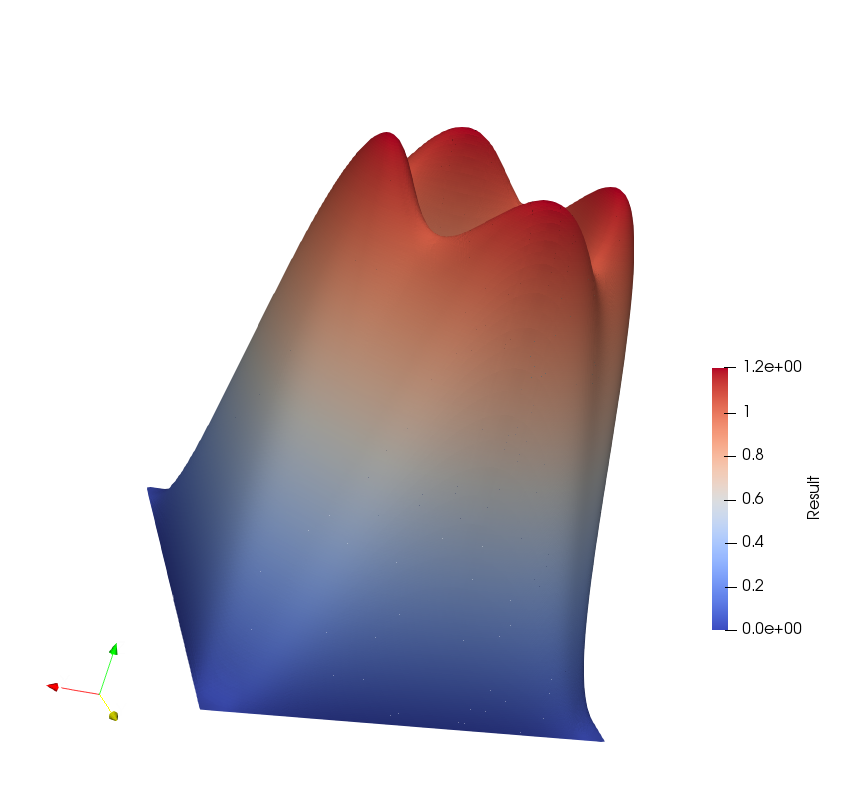
\includegraphics[width=10cm]{stokes_cg_velocities}
	\caption{The magnitude of $\textbf{u}$ plotted at each refinement cycle to (\ref{stokes_eq}) with $\textbf{u}$ given by (\ref{benchmark_u}).}
	\label{fig_stokes_sol}
\end{figure}
\begin{table}[H]
	\begin{center}
		\begin{tabular}{|c|c|c|c|c|c|} \hline
	refinement cycle & cells & dofs & $||p-p_h||_{L^2}$ & $||u-u_h||_{L^2}$ & $||u-u_h||_{H^1}$\\ \hline
0 & 64 & 679 & 5.1016e-02 & 1.0815e-02 & 4.4823e-01\\ \hline
1 & 136 & 1431 & 1.0905e-01 & 9.9175e-03 & 4.1524e-01\\ \hline
2 & 352 & 3635 & 9.7928e-02 & 7.1343e-03 & 2.9415e-01\\ \hline
3 & 856 & 8615 & 2.3689e-02 & 9.6017e-04 & 8.2062e-02\\ \hline
4 & 2128 & 21115 & 1.1988e-02 & 6.2091e-04 & 5.2756e-02\\ \hline
5 & 5128 & 50427 & 2.4096e-03 & 8.6223e-05 & 1.5147e-02\\ \hline
		\end{tabular}
	\caption{Convergence for $\textbf{u}$ and $p$ in different norms.}
	\label{tablebenchmark_convergence}
	\end{center}
\end{table}
The results in the table are illustrated in Figures \ref{fig_pL2}-\ref{fig_uH1}.
\begin{figure}[H]
	\centering
	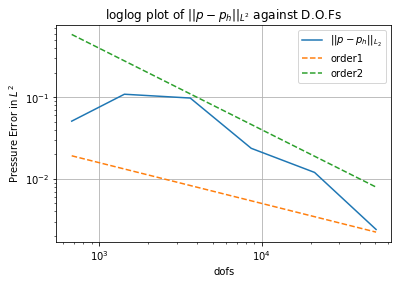
\includegraphics[width=10cm]{p_h_L2}
	\caption{Pressure error in $L^2$: $\left|\left|p-p_h\right|\right|_{L^2}$.}
	\label{fig_pL2}
\end{figure}
\begin{figure}[H]
	\centering
	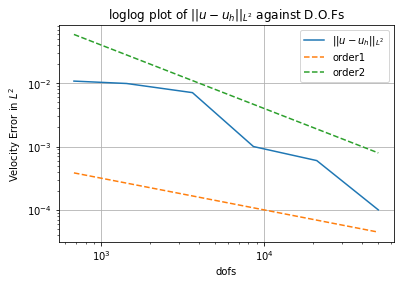
\includegraphics[width=10cm]{u_uh_L2}
	\caption{Velocity error (magnitude) in $L^2$: $\left|\left|u-u_h\right|\right|_{L^2}$.}
	\label{fig_uL2}
\end{figure}
\begin{figure}[H]
	\centering
	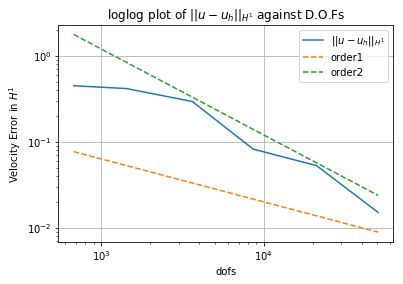
\includegraphics[width=10cm]{u_uh_H1}
	\caption{Velocity error (magnitude) in $H^1$: $\left|\left|u-u_h\right|\right|_{H^1}$.}
	\label{fig_uH1}
\end{figure}
\section{Concluding remarks}\label{sec_conclusion}
\section{Next steps}
\bibliography{biblio_draft}
\bibliographystyle{ieeetr}
\end{document}